\documentclass[1p]{elsarticle_modified}
%\bibliographystyle{elsarticle-num}

%\usepackage[colorlinks]{hyperref}
%\usepackage{abbrmath_seonhwa} %\Abb, \Ascr, \Acal ,\Abf, \Afrak
\usepackage{amsfonts}
\usepackage{amssymb}
\usepackage{amsmath}
\usepackage{amsthm}
\usepackage{scalefnt}
\usepackage{amsbsy}
\usepackage{kotex}
\usepackage{caption}
\usepackage{subfig}
\usepackage{color}
\usepackage{graphicx}
\usepackage{xcolor} %% white, black, red, green, blue, cyan, magenta, yellow
\usepackage{float}
\usepackage{setspace}
\usepackage{hyperref}

\usepackage{tikz}
\usetikzlibrary{arrows}

\usepackage{multirow}
\usepackage{array} % fixed length table
\usepackage{hhline}

%%%%%%%%%%%%%%%%%%%%%
\makeatletter
\renewcommand*\env@matrix[1][\arraystretch]{%
	\edef\arraystretch{#1}%
	\hskip -\arraycolsep
	\let\@ifnextchar\new@ifnextchar
	\array{*\c@MaxMatrixCols c}}
\makeatother %https://tex.stackexchange.com/questions/14071/how-can-i-increase-the-line-spacing-in-a-matrix
%%%%%%%%%%%%%%%

\usepackage[normalem]{ulem}

\newcommand{\msout}[1]{\ifmmode\text{\sout{\ensuremath{#1}}}\else\sout{#1}\fi}
%SOURCE: \msout is \stkout macro in https://tex.stackexchange.com/questions/20609/strikeout-in-math-mode

\newcommand{\cancel}[1]{
	\ifmmode
	{\color{red}\msout{#1}}
	\else
	{\color{red}\sout{#1}}
	\fi
}

\newcommand{\add}[1]{
	{\color{blue}\uwave{#1}}
}

\newcommand{\replace}[2]{
	\ifmmode
	{\color{red}\msout{#1}}{\color{blue}\uwave{#2}}
	\else
	{\color{red}\sout{#1}}{\color{blue}\uwave{#2}}
	\fi
}

\newcommand{\Sol}{\mathcal{S}} %segment
\newcommand{\D}{D} %diagram
\newcommand{\A}{\mathcal{A}} %arc


%%%%%%%%%%%%%%%%%%%%%%%%%%%%%5 test

\def\sl{\operatorname{\textup{SL}}(2,\Cbb)}
\def\psl{\operatorname{\textup{PSL}}(2,\Cbb)}
\def\quan{\mkern 1mu \triangleright \mkern 1mu}

\theoremstyle{definition}
\newtheorem{thm}{Theorem}[section]
\newtheorem{prop}[thm]{Proposition}
\newtheorem{lem}[thm]{Lemma}
\newtheorem{ques}[thm]{Question}
\newtheorem{cor}[thm]{Corollary}
\newtheorem{defn}[thm]{Definition}
\newtheorem{exam}[thm]{Example}
\newtheorem{rmk}[thm]{Remark}
\newtheorem{alg}[thm]{Algorithm}

\newcommand{\I}{\sqrt{-1}}
\begin{document}

%\begin{frontmatter}
%
%\title{Boundary parabolic representations of knots up to 8 crossings}
%
%%% Group authors per affiliation:
%\author{Yunhi Cho} 
%\address{Department of Mathematics, University of Seoul, Seoul, Korea}
%\ead{yhcho@uos.ac.kr}
%
%
%\author{Seonhwa Kim} %\fnref{s_kim}}
%\address{Center for Geometry and Physics, Institute for Basic Science, Pohang, 37673, Korea}
%\ead{ryeona17@ibs.re.kr}
%
%\author{Hyuk Kim}
%\address{Department of Mathematical Sciences, Seoul National University, Seoul 08826, Korea}
%\ead{hyukkim@snu.ac.kr}
%
%\author{Seokbeom Yoon}
%\address{Department of Mathematical Sciences, Seoul National University, Seoul, 08826,  Korea}
%\ead{sbyoon15@snu.ac.kr}
%
%\begin{abstract}
%We find all boundary parabolic representation of knots up to 8 crossings.
%
%\end{abstract}
%\begin{keyword}
%    \MSC[2010] 57M25 
%\end{keyword}
%
%\end{frontmatter}

%\linenumbers
%\tableofcontents
%
\newcommand\colored[1]{\textcolor{white}{\rule[-0.35ex]{0.8em}{1.4ex}}\kern-0.8em\color{red} #1}%
%\newcommand\colored[1]{\textcolor{white}{ #1}\kern-2.17ex	\textcolor{white}{ #1}\kern-1.81ex	\textcolor{white}{ #1}\kern-2.15ex\color{red}#1	}

{\Large $\underline{12a_{1059}~(K12a_{1059})}$}

\setlength{\tabcolsep}{10pt}
\renewcommand{\arraystretch}{1.6}
\vspace{1cm}\begin{tabular}{m{100pt}>{\centering\arraybackslash}m{274pt}}
\multirow{5}{120pt}{
	\centering
	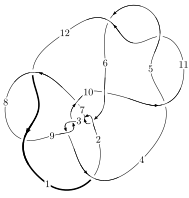
\includegraphics[width=112pt]{../../../GIT/diagram.site/Diagrams/png/1860_12a_1059.png}\\
\ \ \ A knot diagram\footnotemark}&
\allowdisplaybreaks
\textbf{Linearized knot diagam} \\
\cline{2-2}
 &
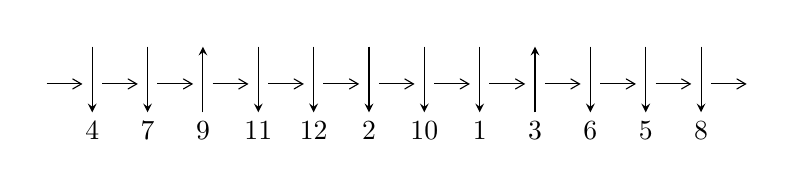
\begin{tikzpicture}[x=20pt, y=17pt]
	% nodes
	\node (C0) at (0, 0) {};
	\node (C1) at (1, 0) {};
	\node (C1U) at (1, +1) {};
	\node (C1D) at (1, -1) {4};

	\node (C2) at (2, 0) {};
	\node (C2U) at (2, +1) {};
	\node (C2D) at (2, -1) {7};

	\node (C3) at (3, 0) {};
	\node (C3U) at (3, +1) {};
	\node (C3D) at (3, -1) {9};

	\node (C4) at (4, 0) {};
	\node (C4U) at (4, +1) {};
	\node (C4D) at (4, -1) {11};

	\node (C5) at (5, 0) {};
	\node (C5U) at (5, +1) {};
	\node (C5D) at (5, -1) {12};

	\node (C6) at (6, 0) {};
	\node (C6U) at (6, +1) {};
	\node (C6D) at (6, -1) {2};

	\node (C7) at (7, 0) {};
	\node (C7U) at (7, +1) {};
	\node (C7D) at (7, -1) {10};

	\node (C8) at (8, 0) {};
	\node (C8U) at (8, +1) {};
	\node (C8D) at (8, -1) {1};

	\node (C9) at (9, 0) {};
	\node (C9U) at (9, +1) {};
	\node (C9D) at (9, -1) {3};

	\node (C10) at (10, 0) {};
	\node (C10U) at (10, +1) {};
	\node (C10D) at (10, -1) {6};

	\node (C11) at (11, 0) {};
	\node (C11U) at (11, +1) {};
	\node (C11D) at (11, -1) {5};

	\node (C12) at (12, 0) {};
	\node (C12U) at (12, +1) {};
	\node (C12D) at (12, -1) {8};
	\node (C13) at (13, 0) {};

	% arrows
	\draw[->,>={angle 60}]
	(C0) edge (C1) (C1) edge (C2) (C2) edge (C3) (C3) edge (C4) (C4) edge (C5) (C5) edge (C6) (C6) edge (C7) (C7) edge (C8) (C8) edge (C9) (C9) edge (C10) (C10) edge (C11) (C11) edge (C12) (C12) edge (C13) ;	\draw[->,>=stealth]
	(C1U) edge (C1D) (C2U) edge (C2D) (C3D) edge (C3U) (C4U) edge (C4D) (C5U) edge (C5D) (C6U) edge (C6D) (C7U) edge (C7D) (C8U) edge (C8D) (C9D) edge (C9U) (C10U) edge (C10D) (C11U) edge (C11D) (C12U) edge (C12D) ;
	\end{tikzpicture} \\
\hhline{~~} \\& 
\textbf{Solving Sequence} \\ \cline{2-2} 
 &
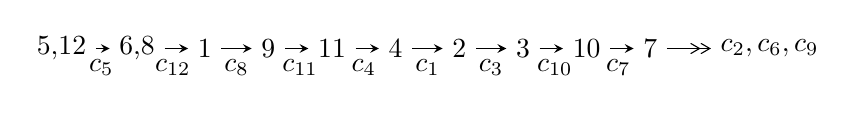
\begin{tikzpicture}[x=23pt, y=7pt]
	% node
	\node (A0) at (-1/8, 0) {5,12};
	\node (A1) at (17/16, 0) {6,8};
	\node (A2) at (17/8, 0) {1};
	\node (A3) at (25/8, 0) {9};
	\node (A4) at (33/8, 0) {11};
	\node (A5) at (41/8, 0) {4};
	\node (A6) at (49/8, 0) {2};
	\node (A7) at (57/8, 0) {3};
	\node (A8) at (65/8, 0) {10};
	\node (A9) at (73/8, 0) {7};
	\node (C1) at (1/2, -1) {$c_{5}$};
	\node (C2) at (13/8, -1) {$c_{12}$};
	\node (C3) at (21/8, -1) {$c_{8}$};
	\node (C4) at (29/8, -1) {$c_{11}$};
	\node (C5) at (37/8, -1) {$c_{4}$};
	\node (C6) at (45/8, -1) {$c_{1}$};
	\node (C7) at (53/8, -1) {$c_{3}$};
	\node (C8) at (61/8, -1) {$c_{10}$};
	\node (C9) at (69/8, -1) {$c_{7}$};
	\node (A10) at (11, 0) {$c_{2},c_{6},c_{9}$};

	% edge
	\draw[->,>=stealth]	
	(A0) edge (A1) (A1) edge (A2) (A2) edge (A3) (A3) edge (A4) (A4) edge (A5) (A5) edge (A6) (A6) edge (A7) (A7) edge (A8) (A8) edge (A9) ;
	\draw[->>,>={angle 60}]	
	(A9) edge (A10);
\end{tikzpicture} \\ 

\end{tabular} \\

\footnotetext{
The image of knot diagram is generated by the software ``\textbf{Draw programme}" developed by Andrew Bartholomew(\url{http://www.layer8.co.uk/maths/draw/index.htm\#Running-draw}), where we modified some parts for our purpose(\url{https://github.com/CATsTAILs/LinksPainter}).
}\phantom \\ \newline 
\centering \textbf{Ideals for irreducible components\footnotemark of $X_{\text{par}}$} 
 
\begin{align*}
I^u_{1}&=\langle 
-6.14828\times10^{28} u^{37}+8.50493\times10^{28} u^{36}+\cdots+2.35548\times10^{29} b+4.37452\times10^{29},\\
\phantom{I^u_{1}}&\phantom{= \langle  }-9.04579\times10^{28} u^{37}+6.37591\times10^{28} u^{36}+\cdots+1.17774\times10^{30} a-2.01495\times10^{30},\\
\phantom{I^u_{1}}&\phantom{= \langle  }u^{38}-3 u^{37}+\cdots+38 u+10\rangle \\
I^u_{2}&=\langle 
2 u^{29} a-3 u^{29}+\cdots+a-9,\;u^{29}+2 u^{28}+\cdots- a+2,\;u^{30}+u^{29}+\cdots- u+1\rangle \\
I^u_{3}&=\langle 
u^4+u^3- u^2+2 b- u+1,\;u^4-2 u^2+a+1,\;u^6-3 u^4+2 u^2+1\rangle \\
\\
I^v_{1}&=\langle 
a,\;b-1,\;v+1\rangle \\
\end{align*}
\raggedright * 4 irreducible components of $\dim_{\mathbb{C}}=0$, with total 105 representations.\\
\footnotetext{All coefficients of polynomials are rational numbers. But the coefficients are sometimes approximated in decimal forms when there is not enough margin.}
\newpage
\renewcommand{\arraystretch}{1}
\centering \section*{I. $I^u_{1}= \langle -6.15\times10^{28} u^{37}+8.50\times10^{28} u^{36}+\cdots+2.36\times10^{29} b+4.37\times10^{29},\;-9.05\times10^{28} u^{37}+6.38\times10^{28} u^{36}+\cdots+1.18\times10^{30} a-2.01\times10^{30},\;u^{38}-3 u^{37}+\cdots+38 u+10 \rangle$}
\flushleft \textbf{(i) Arc colorings}\\
\begin{tabular}{m{7pt} m{180pt} m{7pt} m{180pt} }
\flushright $a_{5}=$&$\begin{pmatrix}1\\0\end{pmatrix}$ \\
\flushright $a_{12}=$&$\begin{pmatrix}0\\u\end{pmatrix}$ \\
\flushright $a_{6}=$&$\begin{pmatrix}1\\u^2\end{pmatrix}$ \\
\flushright $a_{8}=$&$\begin{pmatrix}0.0768064 u^{37}-0.0541369 u^{36}+\cdots+0.400423 u+1.71086\\0.261020 u^{37}-0.361070 u^{36}+\cdots-9.03543 u-1.85717\end{pmatrix}$ \\
\flushright $a_{1}=$&$\begin{pmatrix}0.0395912 u^{37}-0.155029 u^{36}+\cdots+2.31691 u+0.790017\\0.0608242 u^{37}-0.176995 u^{36}+\cdots+0.234757 u-0.377871\end{pmatrix}$ \\
\flushright $a_{9}=$&$\begin{pmatrix}0.140551 u^{37}-0.0696244 u^{36}+\cdots-1.72012 u+2.05575\\0.615558 u^{37}-0.922281 u^{36}+\cdots-22.1653 u-4.52960\end{pmatrix}$ \\
\flushright $a_{11}=$&$\begin{pmatrix}u\\u\end{pmatrix}$ \\
\flushright $a_{4}=$&$\begin{pmatrix}- u^2+1\\- u^2\end{pmatrix}$ \\
\flushright $a_{2}=$&$\begin{pmatrix}-0.00943465 u^{37}-0.0566721 u^{36}+\cdots+2.16486 u+1.21012\\-0.00165545 u^{37}-0.0842333 u^{36}+\cdots+2.11565 u+0.0816969\end{pmatrix}$ \\
\flushright $a_{3}=$&$\begin{pmatrix}-0.100930 u^{37}+0.00413956 u^{36}+\cdots+10.2335 u+3.54732\\-0.209935 u^{37}+0.144189 u^{36}+\cdots+9.07278 u+1.58098\end{pmatrix}$ \\
\flushright $a_{10}=$&$\begin{pmatrix}- u^3+2 u\\- u^5+u^3+u\end{pmatrix}$ \\
\flushright $a_{7}=$&$\begin{pmatrix}0.0740422 u^{37}-0.0468738 u^{36}+\cdots+2.13281 u+2.06658\\0.220414 u^{37}-0.290916 u^{36}+\cdots-6.68558 u-1.35661\end{pmatrix}$\\&\end{tabular}
\flushleft \textbf{(ii) Obstruction class $= -1$}\\~\\
\flushleft \textbf{(iii) Cusp Shapes $= 0.00842304 u^{37}+0.168232 u^{36}+\cdots-43.3018 u-18.3994$}\\~\\
\newpage\renewcommand{\arraystretch}{1}
\flushleft \textbf{(iv) u-Polynomials at the component}\newline \\
\begin{tabular}{m{50pt}|m{274pt}}
Crossings & \hspace{64pt}u-Polynomials at each crossing \\
\hline $$\begin{aligned}c_{1},c_{7}\end{aligned}$$&$\begin{aligned}
&64(64 u^{38}-256 u^{37}+\cdots+15 u-1)
\end{aligned}$\\
\hline $$\begin{aligned}c_{2},c_{6},c_{8}\\c_{12}\end{aligned}$$&$\begin{aligned}
&u^{38}- u^{37}+\cdots+17 u-5
\end{aligned}$\\
\hline $$\begin{aligned}c_{3},c_{9}\end{aligned}$$&$\begin{aligned}
&u^{38}-3 u^{37}+\cdots-834 u+178
\end{aligned}$\\
\hline $$\begin{aligned}c_{4},c_{5},c_{11}\end{aligned}$$&$\begin{aligned}
&u^{38}-3 u^{37}+\cdots+38 u+10
\end{aligned}$\\
\hline $$\begin{aligned}c_{10}\end{aligned}$$&$\begin{aligned}
&u^{38}+9 u^{37}+\cdots-58478 u-6110
\end{aligned}$\\
\hline
\end{tabular}\\~\\
\newpage\renewcommand{\arraystretch}{1}
\flushleft \textbf{(v) Riley Polynomials at the component}\newline \\
\begin{tabular}{m{50pt}|m{274pt}}
Crossings & \hspace{64pt}Riley Polynomials at each crossing \\
\hline $$\begin{aligned}c_{1},c_{7}\end{aligned}$$&$\begin{aligned}
&4096(4096 y^{38}-73728 y^{37}+\cdots-391 y+1)
\end{aligned}$\\
\hline $$\begin{aligned}c_{2},c_{6},c_{8}\\c_{12}\end{aligned}$$&$\begin{aligned}
&y^{38}-19 y^{37}+\cdots-749 y+25
\end{aligned}$\\
\hline $$\begin{aligned}c_{3},c_{9}\end{aligned}$$&$\begin{aligned}
&y^{38}+31 y^{37}+\cdots-180424 y+31684
\end{aligned}$\\
\hline $$\begin{aligned}c_{4},c_{5},c_{11}\end{aligned}$$&$\begin{aligned}
&y^{38}-33 y^{37}+\cdots+896 y+100
\end{aligned}$\\
\hline $$\begin{aligned}c_{10}\end{aligned}$$&$\begin{aligned}
&y^{38}+3 y^{37}+\cdots-52394384 y+37332100
\end{aligned}$\\
\hline
\end{tabular}\\~\\
\newpage\flushleft \textbf{(vi) Complex Volumes and Cusp Shapes}
$$\begin{array}{c|c|c}  
\text{Solutions to }I^u_{1}& \I (\text{vol} + \sqrt{-1}CS) & \text{Cusp shape}\\
 \hline 
\begin{aligned}
u &= -0.832821 + 0.547125 I \\
a &= -0.86558 - 1.12589 I \\
b &= -0.800463 + 0.066461 I\end{aligned}
 & -9.55612 - 8.85033 I & -14.7980 + 4.0064 I \\ \hline\begin{aligned}
u &= -0.832821 - 0.547125 I \\
a &= -0.86558 + 1.12589 I \\
b &= -0.800463 - 0.066461 I\end{aligned}
 & -9.55612 + 8.85033 I & -14.7980 - 4.0064 I \\ \hline\begin{aligned}
u &= \phantom{-}0.758122 + 0.726911 I \\
a &= -0.598468 + 0.868086 I \\
b &= -0.909897 - 0.239586 I\end{aligned}
 & -3.21428 + 2.58317 I & -14.0149 - 7.3951 I \\ \hline\begin{aligned}
u &= \phantom{-}0.758122 - 0.726911 I \\
a &= -0.598468 - 0.868086 I \\
b &= -0.909897 + 0.239586 I\end{aligned}
 & -3.21428 - 2.58317 I & -14.0149 + 7.3951 I \\ \hline\begin{aligned}
u &= -0.254953 + 1.055630 I \\
a &= \phantom{-}0.191552 + 1.039430 I \\
b &= \phantom{-}0.408014 - 0.285100 I\end{aligned}
 & -5.53222 - 1.14690 I & -22.5523 + 4.7902 I \\ \hline\begin{aligned}
u &= -0.254953 - 1.055630 I \\
a &= \phantom{-}0.191552 - 1.039430 I \\
b &= \phantom{-}0.408014 + 0.285100 I\end{aligned}
 & -5.53222 + 1.14690 I & -22.5523 - 4.7902 I \\ \hline\begin{aligned}
u &= \phantom{-}0.377700 + 0.817120 I \\
a &= \phantom{-}0.930523 - 0.994516 I \\
b &= \phantom{-}1.103510 + 0.283151 I\end{aligned}
 & -2.13828 - 7.70452 I & -10.95675 + 8.64865 I \\ \hline\begin{aligned}
u &= \phantom{-}0.377700 - 0.817120 I \\
a &= \phantom{-}0.930523 + 0.994516 I \\
b &= \phantom{-}1.103510 - 0.283151 I\end{aligned}
 & -2.13828 + 7.70452 I & -10.95675 - 8.64865 I \\ \hline\begin{aligned}
u &= -0.304901 + 0.821700 I \\
a &= \phantom{-}1.12461 + 1.25299 I \\
b &= \phantom{-}1.316850 - 0.071626 I\end{aligned}
 & -7.8932 + 13.6180 I & -12.3598 - 8.2723 I \\ \hline\begin{aligned}
u &= -0.304901 - 0.821700 I \\
a &= \phantom{-}1.12461 - 1.25299 I \\
b &= \phantom{-}1.316850 + 0.071626 I\end{aligned}
 & -7.8932 - 13.6180 I & -12.3598 + 8.2723 I\\
 \hline 
 \end{array}$$\newpage$$\begin{array}{c|c|c}  
\text{Solutions to }I^u_{1}& \I (\text{vol} + \sqrt{-1}CS) & \text{Cusp shape}\\
 \hline 
\begin{aligned}
u &= \phantom{-}1.191870 + 0.245310 I \\
a &= -0.597452 - 0.473091 I \\
b &= -1.368890 + 0.168011 I\end{aligned}
 & -0.40005 - 4.16689 I & -6.41890 + 7.16086 I \\ \hline\begin{aligned}
u &= \phantom{-}1.191870 - 0.245310 I \\
a &= -0.597452 + 0.473091 I \\
b &= -1.368890 - 0.168011 I\end{aligned}
 & -0.40005 + 4.16689 I & -6.41890 - 7.16086 I \\ \hline\begin{aligned}
u &= -1.096270 + 0.573423 I \\
a &= -0.932566 - 0.275848 I \\
b &= -1.361430 - 0.074950 I\end{aligned}
 & -8.26421 + 6.83120 I & -17.2078 - 8.7853 I \\ \hline\begin{aligned}
u &= -1.096270 - 0.573423 I \\
a &= -0.932566 + 0.275848 I \\
b &= -1.361430 + 0.074950 I\end{aligned}
 & -8.26421 - 6.83120 I & -17.2078 + 8.7853 I \\ \hline\begin{aligned}
u &= -1.244400 + 0.106432 I \\
a &= -0.500503 + 0.821730 I \\
b &= -1.86027 + 0.16899 I\end{aligned}
 & -2.57552 + 1.10250 I & -12.15322 + 1.49488 I \\ \hline\begin{aligned}
u &= -1.244400 - 0.106432 I \\
a &= -0.500503 - 0.821730 I \\
b &= -1.86027 - 0.16899 I\end{aligned}
 & -2.57552 - 1.10250 I & -12.15322 - 1.49488 I \\ \hline\begin{aligned}
u &= -0.737757\phantom{ +0.000000I} \\
a &= \phantom{-}0.738275\phantom{ +0.000000I} \\
b &= \phantom{-}0.681107\phantom{ +0.000000I}\end{aligned}
 & -1.10279\phantom{ +0.000000I} & -8.36790\phantom{ +0.000000I} \\ \hline\begin{aligned}
u &= \phantom{-}1.288170 + 0.175763 I \\
a &= \phantom{-}0.202837 - 0.012188 I \\
b &= \phantom{-}0.693144 + 1.009580 I\end{aligned}
 & -4.92002 - 2.79762 I & -16.6701 + 3.7773 I \\ \hline\begin{aligned}
u &= \phantom{-}1.288170 - 0.175763 I \\
a &= \phantom{-}0.202837 + 0.012188 I \\
b &= \phantom{-}0.693144 - 1.009580 I\end{aligned}
 & -4.92002 + 2.79762 I & -16.6701 - 3.7773 I \\ \hline\begin{aligned}
u &= \phantom{-}0.062119 + 0.674628 I \\
a &= -1.066350 - 0.720953 I \\
b &= -0.548733 - 0.123939 I\end{aligned}
 & \phantom{-}3.02249 + 0.79229 I & -0.26606 - 2.46888 I\\
 \hline 
 \end{array}$$\newpage$$\begin{array}{c|c|c}  
\text{Solutions to }I^u_{1}& \I (\text{vol} + \sqrt{-1}CS) & \text{Cusp shape}\\
 \hline 
\begin{aligned}
u &= \phantom{-}0.062119 - 0.674628 I \\
a &= -1.066350 + 0.720953 I \\
b &= -0.548733 + 0.123939 I\end{aligned}
 & \phantom{-}3.02249 - 0.79229 I & -0.26606 + 2.46888 I \\ \hline\begin{aligned}
u &= -1.307770 + 0.250331 I \\
a &= \phantom{-}0.089765 + 0.665827 I \\
b &= -0.340750 + 0.653216 I\end{aligned}
 & -1.25101 + 2.53582 I & -5.26256 - 1.09268 I \\ \hline\begin{aligned}
u &= -1.307770 - 0.250331 I \\
a &= \phantom{-}0.089765 - 0.665827 I \\
b &= -0.340750 - 0.653216 I\end{aligned}
 & -1.25101 - 2.53582 I & -5.26256 + 1.09268 I \\ \hline\begin{aligned}
u &= \phantom{-}1.376180 + 0.215614 I \\
a &= -0.007963 - 1.118930 I \\
b &= -0.93586 - 1.62045 I\end{aligned}
 & -4.46084 - 3.77438 I & -17.8969 + 4.8599 I \\ \hline\begin{aligned}
u &= \phantom{-}1.376180 - 0.215614 I \\
a &= -0.007963 + 1.118930 I \\
b &= -0.93586 + 1.62045 I\end{aligned}
 & -4.46084 + 3.77438 I & -17.8969 - 4.8599 I \\ \hline\begin{aligned}
u &= -0.181936 + 0.531158 I \\
a &= -2.10293 + 1.17618 I \\
b &= -0.852184 + 0.229977 I\end{aligned}
 & \phantom{-}0.533620 + 0.994797 I & -12.5887 - 7.1482 I \\ \hline\begin{aligned}
u &= -0.181936 - 0.531158 I \\
a &= -2.10293 - 1.17618 I \\
b &= -0.852184 - 0.229977 I\end{aligned}
 & \phantom{-}0.533620 - 0.994797 I & -12.5887 + 7.1482 I \\ \hline\begin{aligned}
u &= \phantom{-}1.43812 + 0.32819 I \\
a &= \phantom{-}1.024740 + 0.167678 I \\
b &= \phantom{-}3.38065 - 0.99960 I\end{aligned}
 & -13.4573 - 17.7785 I & -15.9854 + 8.9050 I \\ \hline\begin{aligned}
u &= \phantom{-}1.43812 - 0.32819 I \\
a &= \phantom{-}1.024740 - 0.167678 I \\
b &= \phantom{-}3.38065 + 0.99960 I\end{aligned}
 & -13.4573 + 17.7785 I & -15.9854 - 8.9050 I \\ \hline\begin{aligned}
u &= -1.46219 + 0.31744 I \\
a &= \phantom{-}0.886952 - 0.098679 I \\
b &= \phantom{-}3.18286 + 0.68484 I\end{aligned}
 & -8.0205 + 11.8161 I & -14.4580 - 8.0646 I\\
 \hline 
 \end{array}$$\newpage$$\begin{array}{c|c|c}  
\text{Solutions to }I^u_{1}& \I (\text{vol} + \sqrt{-1}CS) & \text{Cusp shape}\\
 \hline 
\begin{aligned}
u &= -1.46219 - 0.31744 I \\
a &= \phantom{-}0.886952 + 0.098679 I \\
b &= \phantom{-}3.18286 - 0.68484 I\end{aligned}
 & -8.0205 - 11.8161 I & -14.4580 + 8.0646 I \\ \hline\begin{aligned}
u &= \phantom{-}1.53956 + 0.03471 I \\
a &= -0.926435 + 0.236128 I \\
b &= -3.32141 + 0.36741 I\end{aligned}
 & -17.7030 + 7.3147 I & -19.0498 - 4.2883 I \\ \hline\begin{aligned}
u &= \phantom{-}1.53956 - 0.03471 I \\
a &= -0.926435 - 0.236128 I \\
b &= -3.32141 - 0.36741 I\end{aligned}
 & -17.7030 - 7.3147 I & -19.0498 + 4.2883 I \\ \hline\begin{aligned}
u &= \phantom{-}1.51262 + 0.38346 I \\
a &= \phantom{-}0.770644 - 0.138564 I \\
b &= \phantom{-}2.50061 - 0.54552 I\end{aligned}
 & -11.37270 - 4.09288 I & -21.9706 + 0. I\phantom{ +0.000000I} \\ \hline\begin{aligned}
u &= \phantom{-}1.51262 - 0.38346 I \\
a &= \phantom{-}0.770644 + 0.138564 I \\
b &= \phantom{-}2.50061 + 0.54552 I\end{aligned}
 & -11.37270 + 4.09288 I & -21.9706 + 0. I\phantom{ +0.000000I} \\ \hline\begin{aligned}
u &= -1.61211\phantom{ +0.000000I} \\
a &= -0.778308\phantom{ +0.000000I} \\
b &= -3.05374\phantom{ +0.000000I}\end{aligned}
 & -12.1718\phantom{ +0.000000I} & -21.8720\phantom{ +0.000000I} \\ \hline\begin{aligned}
u &= -0.184289 + 0.301680 I \\
a &= \phantom{-}1.096640 - 0.014738 I \\
b &= -0.099433 - 0.437896 I\end{aligned}
 & -0.612808 + 0.881258 I & -10.27041 - 7.59569 I \\ \hline\begin{aligned}
u &= -0.184289 - 0.301680 I \\
a &= \phantom{-}1.096640 + 0.014738 I \\
b &= -0.099433 + 0.437896 I\end{aligned}
 & -0.612808 - 0.881258 I & -10.27041 + 7.59569 I\\
 \hline 
 \end{array}$$\newpage\newpage\renewcommand{\arraystretch}{1}
\centering \section*{II. $I^u_{2}= \langle 2 u^{29} a-3 u^{29}+\cdots+a-9,\;u^{29}+2 u^{28}+\cdots- a+2,\;u^{30}+u^{29}+\cdots- u+1 \rangle$}
\flushleft \textbf{(i) Arc colorings}\\
\begin{tabular}{m{7pt} m{180pt} m{7pt} m{180pt} }
\flushright $a_{5}=$&$\begin{pmatrix}1\\0\end{pmatrix}$ \\
\flushright $a_{12}=$&$\begin{pmatrix}0\\u\end{pmatrix}$ \\
\flushright $a_{6}=$&$\begin{pmatrix}1\\u^2\end{pmatrix}$ \\
\flushright $a_{8}=$&$\begin{pmatrix}a\\-\frac{2}{5} u^{29} a+\frac{3}{5} u^{29}+\cdots-\frac{1}{5} a+\frac{9}{5}\end{pmatrix}$ \\
\flushright $a_{1}=$&$\begin{pmatrix}u^{29}+u^{28}+\cdots+3 u-1\\\frac{6}{5} u^{29} a-\frac{1}{5} u^{29}+\cdots+\frac{3}{5} a-\frac{3}{5}\end{pmatrix}$ \\
\flushright $a_{9}=$&$\begin{pmatrix}u^{20}-9 u^{18}+33 u^{16}-60 u^{14}+48 u^{12}+3 u^{10}-25 u^8+2 u^6+9 u^4- u^2-1\\u^{20}-8 u^{18}+26 u^{16}-42 u^{14}+31 u^{12}-2 u^{10}-8 u^8-2 u^6+5 u^4\end{pmatrix}$ \\
\flushright $a_{11}=$&$\begin{pmatrix}u\\u\end{pmatrix}$ \\
\flushright $a_{4}=$&$\begin{pmatrix}- u^2+1\\- u^2\end{pmatrix}$ \\
\flushright $a_{2}=$&$\begin{pmatrix}\frac{1}{5} u^{29} a+\frac{9}{5} u^{29}+\cdots+\frac{3}{5} a+\frac{2}{5}\\\frac{4}{5} u^{29} a+\frac{6}{5} u^{29}+\cdots+\frac{2}{5} a+\frac{3}{5}\end{pmatrix}$ \\
\flushright $a_{3}=$&$\begin{pmatrix}u^{21}-10 u^{19}+\cdots-6 u^3- u\\u^{23}-9 u^{21}+\cdots-2 u^3- u\end{pmatrix}$ \\
\flushright $a_{10}=$&$\begin{pmatrix}- u^3+2 u\\- u^5+u^3+u\end{pmatrix}$ \\
\flushright $a_{7}=$&$\begin{pmatrix}\frac{3}{5} u^{29} a+\frac{3}{5} u^{29}+\cdots+\frac{9}{5} a-\frac{1}{5}\\\frac{7}{5} u^{29} a+\frac{2}{5} u^{29}+\cdots+\frac{6}{5} a+\frac{6}{5}\end{pmatrix}$\\&\end{tabular}
\flushleft \textbf{(ii) Obstruction class $= -1$}\\~\\
\flushleft \textbf{(iii) Cusp Shapes $= 4 u^{28}-52 u^{26}+4 u^{25}+292 u^{24}-48 u^{23}-912 u^{22}+244 u^{21}+1684 u^{20}-672 u^{19}-1752 u^{18}+1056 u^{17}+752 u^{16}-896 u^{15}+212 u^{14}+332 u^{13}-180 u^{12}-64 u^{11}-156 u^{10}+112 u^9+96 u^8-64 u^7+20 u^6+8 u^5-8 u^4-20 u^3+12 u-14$}\\~\\
\newpage\renewcommand{\arraystretch}{1}
\flushleft \textbf{(iv) u-Polynomials at the component}\newline \\
\begin{tabular}{m{50pt}|m{274pt}}
Crossings & \hspace{64pt}u-Polynomials at each crossing \\
\hline $$\begin{aligned}c_{1},c_{7}\end{aligned}$$&$\begin{aligned}
&25(25 u^{60}+175 u^{59}+\cdots-6914990 u+533119)
\end{aligned}$\\
\hline $$\begin{aligned}c_{2},c_{6},c_{8}\\c_{12}\end{aligned}$$&$\begin{aligned}
&u^{60}- u^{59}+\cdots+2 u^2+1
\end{aligned}$\\
\hline $$\begin{aligned}c_{3},c_{9}\end{aligned}$$&$\begin{aligned}
&(u^{30}+u^{29}+\cdots+u+1)^{2}
\end{aligned}$\\
\hline $$\begin{aligned}c_{4},c_{5},c_{11}\end{aligned}$$&$\begin{aligned}
&(u^{30}+u^{29}+\cdots- u+1)^{2}
\end{aligned}$\\
\hline $$\begin{aligned}c_{10}\end{aligned}$$&$\begin{aligned}
&(u^{30}-3 u^{29}+\cdots- u+1)^{2}
\end{aligned}$\\
\hline
\end{tabular}\\~\\
\newpage\renewcommand{\arraystretch}{1}
\flushleft \textbf{(v) Riley Polynomials at the component}\newline \\
\begin{tabular}{m{50pt}|m{274pt}}
Crossings & \hspace{64pt}Riley Polynomials at each crossing \\
\hline $$\begin{aligned}c_{1},c_{7}\end{aligned}$$&$\begin{aligned}
&625\\
&\cdot(625 y^{60}-20625 y^{59}+\cdots-3671828841416 y+284215868161)
\end{aligned}$\\
\hline $$\begin{aligned}c_{2},c_{6},c_{8}\\c_{12}\end{aligned}$$&$\begin{aligned}
&y^{60}-41 y^{59}+\cdots+4 y+1
\end{aligned}$\\
\hline $$\begin{aligned}c_{3},c_{9}\end{aligned}$$&$\begin{aligned}
&(y^{30}+25 y^{29}+\cdots+3 y+1)^{2}
\end{aligned}$\\
\hline $$\begin{aligned}c_{4},c_{5},c_{11}\end{aligned}$$&$\begin{aligned}
&(y^{30}-27 y^{29}+\cdots+3 y+1)^{2}
\end{aligned}$\\
\hline $$\begin{aligned}c_{10}\end{aligned}$$&$\begin{aligned}
&(y^{30}+y^{29}+\cdots- y+1)^{2}
\end{aligned}$\\
\hline
\end{tabular}\\~\\
\newpage\flushleft \textbf{(vi) Complex Volumes and Cusp Shapes}
$$\begin{array}{c|c|c}  
\text{Solutions to }I^u_{2}& \I (\text{vol} + \sqrt{-1}CS) & \text{Cusp shape}\\
 \hline 
\begin{aligned}
u &= \phantom{-}1.006930 + 0.206480 I \\
a &= \phantom{-}1.106440 + 0.089649 I \\
b &= \phantom{-}0.700491 + 0.212708 I\end{aligned}
 & -4.85148 - 3.89629 I & -11.54228 + 4.15365 I \\ \hline\begin{aligned}
u &= \phantom{-}1.006930 + 0.206480 I \\
a &= -0.062835 - 0.576338 I \\
b &= \phantom{-}0.716396 + 0.426617 I\end{aligned}
 & -4.85148 - 3.89629 I & -11.54228 + 4.15365 I \\ \hline\begin{aligned}
u &= \phantom{-}1.006930 - 0.206480 I \\
a &= \phantom{-}1.106440 - 0.089649 I \\
b &= \phantom{-}0.700491 - 0.212708 I\end{aligned}
 & -4.85148 + 3.89629 I & -11.54228 - 4.15365 I \\ \hline\begin{aligned}
u &= \phantom{-}1.006930 - 0.206480 I \\
a &= -0.062835 + 0.576338 I \\
b &= \phantom{-}0.716396 - 0.426617 I\end{aligned}
 & -4.85148 + 3.89629 I & -11.54228 - 4.15365 I \\ \hline\begin{aligned}
u &= -0.832034 + 0.169903 I \\
a &= \phantom{-}0.837632 + 0.478792 I \\
b &= \phantom{-}0.728628 - 0.013221 I\end{aligned}
 & -1.081760 - 0.029483 I & -7.62798 - 0.47071 I \\ \hline\begin{aligned}
u &= -0.832034 + 0.169903 I \\
a &= \phantom{-}0.541539 - 0.269552 I \\
b &= \phantom{-}0.764830 - 0.085001 I\end{aligned}
 & -1.081760 - 0.029483 I & -7.62798 - 0.47071 I \\ \hline\begin{aligned}
u &= -0.832034 - 0.169903 I \\
a &= \phantom{-}0.837632 - 0.478792 I \\
b &= \phantom{-}0.728628 + 0.013221 I\end{aligned}
 & -1.081760 + 0.029483 I & -7.62798 + 0.47071 I \\ \hline\begin{aligned}
u &= -0.832034 - 0.169903 I \\
a &= \phantom{-}0.541539 + 0.269552 I \\
b &= \phantom{-}0.764830 + 0.085001 I\end{aligned}
 & -1.081760 + 0.029483 I & -7.62798 + 0.47071 I \\ \hline\begin{aligned}
u &= \phantom{-}0.266850 + 0.721202 I \\
a &= \phantom{-}1.39335 + 0.53326 I \\
b &= \phantom{-}0.755461 + 0.165673 I\end{aligned}
 & -3.58803 - 7.69168 I & -9.96957 + 6.90287 I \\ \hline\begin{aligned}
u &= \phantom{-}0.266850 + 0.721202 I \\
a &= -1.34228 + 1.44900 I \\
b &= -1.176110 + 0.077817 I\end{aligned}
 & -3.58803 - 7.69168 I & -9.96957 + 6.90287 I\\
 \hline 
 \end{array}$$\newpage$$\begin{array}{c|c|c}  
\text{Solutions to }I^u_{2}& \I (\text{vol} + \sqrt{-1}CS) & \text{Cusp shape}\\
 \hline 
\begin{aligned}
u &= \phantom{-}0.266850 - 0.721202 I \\
a &= \phantom{-}1.39335 - 0.53326 I \\
b &= \phantom{-}0.755461 - 0.165673 I\end{aligned}
 & -3.58803 + 7.69168 I & -9.96957 - 6.90287 I \\ \hline\begin{aligned}
u &= \phantom{-}0.266850 - 0.721202 I \\
a &= -1.34228 - 1.44900 I \\
b &= -1.176110 - 0.077817 I\end{aligned}
 & -3.58803 + 7.69168 I & -9.96957 - 6.90287 I \\ \hline\begin{aligned}
u &= \phantom{-}0.703536 + 0.310326 I \\
a &= \phantom{-}0.375402 + 1.132660 I \\
b &= \phantom{-}0.726738 + 0.185162 I\end{aligned}
 & -5.20234 + 3.85600 I & -12.77500 - 2.05029 I \\ \hline\begin{aligned}
u &= \phantom{-}0.703536 + 0.310326 I \\
a &= \phantom{-}1.35245 - 1.17888 I \\
b &= \phantom{-}0.727398 - 0.288938 I\end{aligned}
 & -5.20234 + 3.85600 I & -12.77500 - 2.05029 I \\ \hline\begin{aligned}
u &= \phantom{-}0.703536 - 0.310326 I \\
a &= \phantom{-}0.375402 - 1.132660 I \\
b &= \phantom{-}0.726738 - 0.185162 I\end{aligned}
 & -5.20234 - 3.85600 I & -12.77500 + 2.05029 I \\ \hline\begin{aligned}
u &= \phantom{-}0.703536 - 0.310326 I \\
a &= \phantom{-}1.35245 + 1.17888 I \\
b &= \phantom{-}0.727398 + 0.288938 I\end{aligned}
 & -5.20234 - 3.85600 I & -12.77500 + 2.05029 I \\ \hline\begin{aligned}
u &= -0.228391 + 0.710789 I \\
a &= \phantom{-}0.824807 - 0.489046 I \\
b &= \phantom{-}0.348965 + 0.017513 I\end{aligned}
 & \phantom{-}0.89469 + 3.64220 I & -4.89571 - 4.72167 I \\ \hline\begin{aligned}
u &= -0.228391 + 0.710789 I \\
a &= -0.98019 - 1.20859 I \\
b &= -1.058380 + 0.072042 I\end{aligned}
 & \phantom{-}0.89469 + 3.64220 I & -4.89571 - 4.72167 I \\ \hline\begin{aligned}
u &= -0.228391 - 0.710789 I \\
a &= \phantom{-}0.824807 + 0.489046 I \\
b &= \phantom{-}0.348965 - 0.017513 I\end{aligned}
 & \phantom{-}0.89469 - 3.64220 I & -4.89571 + 4.72167 I \\ \hline\begin{aligned}
u &= -0.228391 - 0.710789 I \\
a &= -0.98019 + 1.20859 I \\
b &= -1.058380 - 0.072042 I\end{aligned}
 & \phantom{-}0.89469 - 3.64220 I & -4.89571 + 4.72167 I\\
 \hline 
 \end{array}$$\newpage$$\begin{array}{c|c|c}  
\text{Solutions to }I^u_{2}& \I (\text{vol} + \sqrt{-1}CS) & \text{Cusp shape}\\
 \hline 
\begin{aligned}
u &= \phantom{-}0.169829 + 0.699155 I \\
a &= -0.27507 + 1.43355 I \\
b &= -0.982543 + 0.271641 I\end{aligned}
 & -2.35081 + 0.37332 I & -7.79326 + 0.53471 I \\ \hline\begin{aligned}
u &= \phantom{-}0.169829 + 0.699155 I \\
a &= -0.129943 - 0.165869 I \\
b &= -0.264670 - 0.891458 I\end{aligned}
 & -2.35081 + 0.37332 I & -7.79326 + 0.53471 I \\ \hline\begin{aligned}
u &= \phantom{-}0.169829 - 0.699155 I \\
a &= -0.27507 - 1.43355 I \\
b &= -0.982543 - 0.271641 I\end{aligned}
 & -2.35081 - 0.37332 I & -7.79326 - 0.53471 I \\ \hline\begin{aligned}
u &= \phantom{-}0.169829 - 0.699155 I \\
a &= -0.129943 + 0.165869 I \\
b &= -0.264670 + 0.891458 I\end{aligned}
 & -2.35081 - 0.37332 I & -7.79326 - 0.53471 I \\ \hline\begin{aligned}
u &= -0.379833 + 0.540597 I \\
a &= \phantom{-}1.91795 + 1.04697 I \\
b &= \phantom{-}1.285490 + 0.431592 I\end{aligned}
 & -8.44109 + 1.73295 I & -15.3118 - 4.0988 I \\ \hline\begin{aligned}
u &= -0.379833 + 0.540597 I \\
a &= -0.70200 - 2.19064 I \\
b &= -0.195589 - 0.222195 I\end{aligned}
 & -8.44109 + 1.73295 I & -15.3118 - 4.0988 I \\ \hline\begin{aligned}
u &= -0.379833 - 0.540597 I \\
a &= \phantom{-}1.91795 - 1.04697 I \\
b &= \phantom{-}1.285490 - 0.431592 I\end{aligned}
 & -8.44109 - 1.73295 I & -15.3118 + 4.0988 I \\ \hline\begin{aligned}
u &= -0.379833 - 0.540597 I \\
a &= -0.70200 + 2.19064 I \\
b &= -0.195589 + 0.222195 I\end{aligned}
 & -8.44109 - 1.73295 I & -15.3118 + 4.0988 I \\ \hline\begin{aligned}
u &= \phantom{-}1.351750 + 0.104838 I \\
a &= \phantom{-}0.918606 - 0.092731 I \\
b &= \phantom{-}3.58585 - 0.17980 I\end{aligned}
 & -6.82103 - 0.39832 I & -11.93478 - 1.62643 I \\ \hline\begin{aligned}
u &= \phantom{-}1.351750 + 0.104838 I \\
a &= -0.387734 + 0.353048 I \\
b &= \phantom{-}0.384313 - 0.303024 I\end{aligned}
 & -6.82103 - 0.39832 I & -11.93478 - 1.62643 I\\
 \hline 
 \end{array}$$\newpage$$\begin{array}{c|c|c}  
\text{Solutions to }I^u_{2}& \I (\text{vol} + \sqrt{-1}CS) & \text{Cusp shape}\\
 \hline 
\begin{aligned}
u &= \phantom{-}1.351750 - 0.104838 I \\
a &= \phantom{-}0.918606 + 0.092731 I \\
b &= \phantom{-}3.58585 + 0.17980 I\end{aligned}
 & -6.82103 + 0.39832 I & -11.93478 + 1.62643 I \\ \hline\begin{aligned}
u &= \phantom{-}1.351750 - 0.104838 I \\
a &= -0.387734 - 0.353048 I \\
b &= \phantom{-}0.384313 + 0.303024 I\end{aligned}
 & -6.82103 + 0.39832 I & -11.93478 + 1.62643 I \\ \hline\begin{aligned}
u &= -1.363600 + 0.194579 I \\
a &= -0.776181 - 0.304313 I \\
b &= -3.24492 + 0.96961 I\end{aligned}
 & -8.06303 + 3.51597 I & -14.7951 - 5.1228 I \\ \hline\begin{aligned}
u &= -1.363600 + 0.194579 I \\
a &= \phantom{-}0.815095 - 0.090094 I \\
b &= \phantom{-}3.99423 + 2.25543 I\end{aligned}
 & -8.06303 + 3.51597 I & -14.7951 - 5.1228 I \\ \hline\begin{aligned}
u &= -1.363600 - 0.194579 I \\
a &= -0.776181 + 0.304313 I \\
b &= -3.24492 - 0.96961 I\end{aligned}
 & -8.06303 - 3.51597 I & -14.7951 + 5.1228 I \\ \hline\begin{aligned}
u &= -1.363600 - 0.194579 I \\
a &= \phantom{-}0.815095 + 0.090094 I \\
b &= \phantom{-}3.99423 - 2.25543 I\end{aligned}
 & -8.06303 - 3.51597 I & -14.7951 + 5.1228 I \\ \hline\begin{aligned}
u &= -1.360050 + 0.270550 I \\
a &= -0.801459 - 0.128170 I \\
b &= -3.02150 - 2.03985 I\end{aligned}
 & -7.18585 + 3.12979 I & -12.91872 - 1.86186 I \\ \hline\begin{aligned}
u &= -1.360050 + 0.270550 I \\
a &= \phantom{-}0.231493 - 0.068682 I \\
b &= -0.845504 + 1.046880 I\end{aligned}
 & -7.18585 + 3.12979 I & -12.91872 - 1.86186 I \\ \hline\begin{aligned}
u &= -1.360050 - 0.270550 I \\
a &= -0.801459 + 0.128170 I \\
b &= -3.02150 + 2.03985 I\end{aligned}
 & -7.18585 - 3.12979 I & -12.91872 + 1.86186 I \\ \hline\begin{aligned}
u &= -1.360050 - 0.270550 I \\
a &= \phantom{-}0.231493 + 0.068682 I \\
b &= -0.845504 - 1.046880 I\end{aligned}
 & -7.18585 - 3.12979 I & -12.91872 + 1.86186 I\\
 \hline 
 \end{array}$$\newpage$$\begin{array}{c|c|c}  
\text{Solutions to }I^u_{2}& \I (\text{vol} + \sqrt{-1}CS) & \text{Cusp shape}\\
 \hline 
\begin{aligned}
u &= \phantom{-}1.39028 + 0.28253 I \\
a &= -0.893925 - 0.133521 I \\
b &= -3.12549 + 0.97945 I\end{aligned}
 & -4.25247 - 7.24749 I & -9.92864 + 5.63452 I \\ \hline\begin{aligned}
u &= \phantom{-}1.39028 + 0.28253 I \\
a &= \phantom{-}0.082294 + 0.578132 I \\
b &= \phantom{-}0.382082 + 0.552723 I\end{aligned}
 & -4.25247 - 7.24749 I & -9.92864 + 5.63452 I \\ \hline\begin{aligned}
u &= \phantom{-}1.39028 - 0.28253 I \\
a &= -0.893925 + 0.133521 I \\
b &= -3.12549 - 0.97945 I\end{aligned}
 & -4.25247 + 7.24749 I & -9.92864 - 5.63452 I \\ \hline\begin{aligned}
u &= \phantom{-}1.39028 - 0.28253 I \\
a &= \phantom{-}0.082294 - 0.578132 I \\
b &= \phantom{-}0.382082 - 0.552723 I\end{aligned}
 & -4.25247 + 7.24749 I & -9.92864 - 5.63452 I \\ \hline\begin{aligned}
u &= -1.42059 + 0.09196 I \\
a &= \phantom{-}1.085040 + 0.253869 I \\
b &= \phantom{-}3.38504 + 0.97196 I\end{aligned}
 & -11.61500 - 2.69486 I & -17.4134 + 2.4278 I \\ \hline\begin{aligned}
u &= -1.42059 + 0.09196 I \\
a &= -0.272288 - 0.773726 I \\
b &= \phantom{-}0.134709 - 1.163670 I\end{aligned}
 & -11.61500 - 2.69486 I & -17.4134 + 2.4278 I \\ \hline\begin{aligned}
u &= -1.42059 - 0.09196 I \\
a &= \phantom{-}1.085040 - 0.253869 I \\
b &= \phantom{-}3.38504 - 0.97196 I\end{aligned}
 & -11.61500 + 2.69486 I & -17.4134 - 2.4278 I \\ \hline\begin{aligned}
u &= -1.42059 - 0.09196 I \\
a &= -0.272288 + 0.773726 I \\
b &= \phantom{-}0.134709 + 1.163670 I\end{aligned}
 & -11.61500 + 2.69486 I & -17.4134 - 2.4278 I \\ \hline\begin{aligned}
u &= -1.40881 + 0.28598 I \\
a &= \phantom{-}0.178934 - 0.868467 I \\
b &= \phantom{-}1.10783 - 1.01091 I\end{aligned}
 & -8.9306 + 11.3520 I & -14.5534 - 7.3132 I \\ \hline\begin{aligned}
u &= -1.40881 + 0.28598 I \\
a &= -1.104570 + 0.226478 I \\
b &= -3.42336 - 0.88023 I\end{aligned}
 & -8.9306 + 11.3520 I & -14.5534 - 7.3132 I\\
 \hline 
 \end{array}$$\newpage$$\begin{array}{c|c|c}  
\text{Solutions to }I^u_{2}& \I (\text{vol} + \sqrt{-1}CS) & \text{Cusp shape}\\
 \hline 
\begin{aligned}
u &= -1.40881 - 0.28598 I \\
a &= \phantom{-}0.178934 + 0.868467 I \\
b &= \phantom{-}1.10783 + 1.01091 I\end{aligned}
 & -8.9306 - 11.3520 I & -14.5534 + 7.3132 I \\ \hline\begin{aligned}
u &= -1.40881 - 0.28598 I \\
a &= -1.104570 - 0.226478 I \\
b &= -3.42336 + 0.88023 I\end{aligned}
 & -8.9306 - 11.3520 I & -14.5534 + 7.3132 I \\ \hline\begin{aligned}
u &= \phantom{-}1.42434 + 0.20546 I \\
a &= \phantom{-}1.029910 + 0.423098 I \\
b &= \phantom{-}3.20762 - 0.64618 I\end{aligned}
 & -14.1830 - 4.4767 I & -19.0263 + 3.5734 I \\ \hline\begin{aligned}
u &= \phantom{-}1.42434 + 0.20546 I \\
a &= -1.070140 + 0.500011 I \\
b &= -2.72487 + 1.14691 I\end{aligned}
 & -14.1830 - 4.4767 I & -19.0263 + 3.5734 I \\ \hline\begin{aligned}
u &= \phantom{-}1.42434 - 0.20546 I \\
a &= \phantom{-}1.029910 - 0.423098 I \\
b &= \phantom{-}3.20762 + 0.64618 I\end{aligned}
 & -14.1830 + 4.4767 I & -19.0263 - 3.5734 I \\ \hline\begin{aligned}
u &= \phantom{-}1.42434 - 0.20546 I \\
a &= -1.070140 - 0.500011 I \\
b &= -2.72487 - 1.14691 I\end{aligned}
 & -14.1830 + 4.4767 I & -19.0263 - 3.5734 I \\ \hline\begin{aligned}
u &= \phantom{-}0.179795 + 0.471439 I \\
a &= \phantom{-}1.11876 - 1.63717 I \\
b &= \phantom{-}1.72380 - 0.44845 I\end{aligned}
 & -3.15470 - 0.99510 I & -9.51394 + 6.82295 I \\ \hline\begin{aligned}
u &= \phantom{-}0.179795 + 0.471439 I \\
a &= -0.51110 + 2.18288 I \\
b &= -0.096933 - 0.875944 I\end{aligned}
 & -3.15470 - 0.99510 I & -9.51394 + 6.82295 I \\ \hline\begin{aligned}
u &= \phantom{-}0.179795 - 0.471439 I \\
a &= \phantom{-}1.11876 + 1.63717 I \\
b &= \phantom{-}1.72380 + 0.44845 I\end{aligned}
 & -3.15470 + 0.99510 I & -9.51394 - 6.82295 I \\ \hline\begin{aligned}
u &= \phantom{-}0.179795 - 0.471439 I \\
a &= -0.51110 - 2.18288 I \\
b &= -0.096933 + 0.875944 I\end{aligned}
 & -3.15470 + 0.99510 I & -9.51394 - 6.82295 I\\
 \hline 
 \end{array}$$\newpage\newpage\renewcommand{\arraystretch}{1}
\centering \section*{III. $I^u_{3}= \langle u^4+u^3- u^2+2 b- u+1,\;u^4-2 u^2+a+1,\;u^6-3 u^4+2 u^2+1 \rangle$}
\flushleft \textbf{(i) Arc colorings}\\
\begin{tabular}{m{7pt} m{180pt} m{7pt} m{180pt} }
\flushright $a_{5}=$&$\begin{pmatrix}1\\0\end{pmatrix}$ \\
\flushright $a_{12}=$&$\begin{pmatrix}0\\u\end{pmatrix}$ \\
\flushright $a_{6}=$&$\begin{pmatrix}1\\u^2\end{pmatrix}$ \\
\flushright $a_{8}=$&$\begin{pmatrix}- u^4+2 u^2-1\\-\frac{1}{2} u^4-\frac{1}{2} u^3+\cdots+\frac{1}{2} u-\frac{1}{2}\end{pmatrix}$ \\
\flushright $a_{1}=$&$\begin{pmatrix}- u^5+3 u^3-2 u\\- u^5-\frac{1}{2} u^4+2 u^3+u^2+\frac{1}{2} u\end{pmatrix}$ \\
\flushright $a_{9}=$&$\begin{pmatrix}-2 u^4+4 u^2-2\\-2 u^4- u^3+2 u^2+u\end{pmatrix}$ \\
\flushright $a_{11}=$&$\begin{pmatrix}u\\u\end{pmatrix}$ \\
\flushright $a_{4}=$&$\begin{pmatrix}- u^2+1\\- u^2\end{pmatrix}$ \\
\flushright $a_{2}=$&$\begin{pmatrix}-\frac{3}{2} u^5+4 u^3+\cdots-\frac{5}{2} u+\frac{1}{2}\\-\frac{3}{2} u^5-\frac{1}{2} u^4+\cdots+\frac{1}{2} u^2+\frac{1}{2} u\end{pmatrix}$ \\
\flushright $a_{3}=$&$\begin{pmatrix}-2 u^5+6 u^3- u^2-4 u+1\\-2 u^5- u^4+4 u^3+u^2\end{pmatrix}$ \\
\flushright $a_{10}=$&$\begin{pmatrix}- u^3+2 u\\- u^5+u^3+u\end{pmatrix}$ \\
\flushright $a_{7}=$&$\begin{pmatrix}- u^4+\frac{1}{2} u^3+2 u^2- u-\frac{1}{2}\\\frac{1}{2} u^5- u^4- u^3+\frac{3}{2} u^2\end{pmatrix}$\\&\end{tabular}
\flushleft \textbf{(ii) Obstruction class $= 1$}\\~\\
\flushleft \textbf{(iii) Cusp Shapes $= 4 u^4-8 u^2-8$}\\~\\
\newpage\renewcommand{\arraystretch}{1}
\flushleft \textbf{(iv) u-Polynomials at the component}\newline \\
\begin{tabular}{m{50pt}|m{274pt}}
Crossings & \hspace{64pt}u-Polynomials at each crossing \\
\hline $$\begin{aligned}c_{1},c_{7}\end{aligned}$$&$\begin{aligned}
&64(64 u^6-192 u^5+256 u^4-192 u^3+92 u^2-28 u+5)
\end{aligned}$\\
\hline $$\begin{aligned}c_{2},c_{3},c_{6}\\c_{8},c_{9},c_{12}\end{aligned}$$&$\begin{aligned}
&(u^2+1)^3
\end{aligned}$\\
\hline $$\begin{aligned}c_{4},c_{5},c_{11}\end{aligned}$$&$\begin{aligned}
&u^6-3 u^4+2 u^2+1
\end{aligned}$\\
\hline $$\begin{aligned}c_{10}\end{aligned}$$&$\begin{aligned}
&u^6+u^4+2 u^2+1
\end{aligned}$\\
\hline
\end{tabular}\\~\\
\newpage\renewcommand{\arraystretch}{1}
\flushleft \textbf{(v) Riley Polynomials at the component}\newline \\
\begin{tabular}{m{50pt}|m{274pt}}
Crossings & \hspace{64pt}Riley Polynomials at each crossing \\
\hline $$\begin{aligned}c_{1},c_{7}\end{aligned}$$&$\begin{aligned}
&4096(4096 y^6-4096 y^5+3584 y^4+128 y^3+272 y^2+136 y+25)
\end{aligned}$\\
\hline $$\begin{aligned}c_{2},c_{3},c_{6}\\c_{8},c_{9},c_{12}\end{aligned}$$&$\begin{aligned}
&(y+1)^6
\end{aligned}$\\
\hline $$\begin{aligned}c_{4},c_{5},c_{11}\end{aligned}$$&$\begin{aligned}
&(y^3-3 y^2+2 y+1)^2
\end{aligned}$\\
\hline $$\begin{aligned}c_{10}\end{aligned}$$&$\begin{aligned}
&(y^3+y^2+2 y+1)^2
\end{aligned}$\\
\hline
\end{tabular}\\~\\
\newpage\flushleft \textbf{(vi) Complex Volumes and Cusp Shapes}
$$\begin{array}{c|c|c}  
\text{Solutions to }I^u_{3}& \I (\text{vol} + \sqrt{-1}CS) & \text{Cusp shape}\\
 \hline 
\begin{aligned}
u &= \phantom{-}1.307140 + 0.215080 I \\
a &= -0.122561 - 0.744862 I \\
b &= -1.26489 - 1.09229 I\end{aligned}
 & -3.02413 - 2.82812 I & -11.50976 + 2.97945 I \\ \hline\begin{aligned}
u &= \phantom{-}1.307140 - 0.215080 I \\
a &= -0.122561 + 0.744862 I \\
b &= -1.26489 + 1.09229 I\end{aligned}
 & -3.02413 + 2.82812 I & -11.50976 - 2.97945 I \\ \hline\begin{aligned}
u &= -1.307140 + 0.215080 I \\
a &= -0.122561 + 0.744862 I \\
b &= -0.520029 + 0.214851 I\end{aligned}
 & -3.02413 + 2.82812 I & -11.50976 - 2.97945 I \\ \hline\begin{aligned}
u &= -1.307140 - 0.215080 I \\
a &= -0.122561 - 0.744862 I \\
b &= -0.520029 - 0.214851 I\end{aligned}
 & -3.02413 - 2.82812 I & -11.50976 + 2.97945 I \\ \hline\begin{aligned}
u &= \phantom{-0.000000 -}0.569840 I \\
a &= -1.75488\phantom{ +0.000000I} \\
b &= -0.715080 + 0.377439 I\end{aligned}
 & \phantom{-}1.11345\phantom{ +0.000000I} & -4.98050\phantom{ +0.000000I} \\ \hline\begin{aligned}
u &= \phantom{-0.000000 } -0.569840 I \\
a &= -1.75488\phantom{ +0.000000I} \\
b &= -0.715080 - 0.377439 I\end{aligned}
 & \phantom{-}1.11345\phantom{ +0.000000I} & -4.98050\phantom{ +0.000000I}\\
 \hline 
 \end{array}$$\newpage\newpage\renewcommand{\arraystretch}{1}
\centering \section*{IV. $I^v_{1}= \langle a,\;b-1,\;v+1 \rangle$}
\flushleft \textbf{(i) Arc colorings}\\
\begin{tabular}{m{7pt} m{180pt} m{7pt} m{180pt} }
\flushright $a_{5}=$&$\begin{pmatrix}1\\0\end{pmatrix}$ \\
\flushright $a_{12}=$&$\begin{pmatrix}-1\\0\end{pmatrix}$ \\
\flushright $a_{6}=$&$\begin{pmatrix}1\\0\end{pmatrix}$ \\
\flushright $a_{8}=$&$\begin{pmatrix}0\\1\end{pmatrix}$ \\
\flushright $a_{1}=$&$\begin{pmatrix}-1\\-1\end{pmatrix}$ \\
\flushright $a_{9}=$&$\begin{pmatrix}-1\\0\end{pmatrix}$ \\
\flushright $a_{11}=$&$\begin{pmatrix}-1\\0\end{pmatrix}$ \\
\flushright $a_{4}=$&$\begin{pmatrix}1\\0\end{pmatrix}$ \\
\flushright $a_{2}=$&$\begin{pmatrix}0\\-1\end{pmatrix}$ \\
\flushright $a_{3}=$&$\begin{pmatrix}1\\0\end{pmatrix}$ \\
\flushright $a_{10}=$&$\begin{pmatrix}-1\\0\end{pmatrix}$ \\
\flushright $a_{7}=$&$\begin{pmatrix}1\\1\end{pmatrix}$\\&\end{tabular}
\flushleft \textbf{(ii) Obstruction class $= 1$}\\~\\
\flushleft \textbf{(iii) Cusp Shapes $= -12$}\\~\\
\newpage\renewcommand{\arraystretch}{1}
\flushleft \textbf{(iv) u-Polynomials at the component}\newline \\
\begin{tabular}{m{50pt}|m{274pt}}
Crossings & \hspace{64pt}u-Polynomials at each crossing \\
\hline $$\begin{aligned}c_{1},c_{2},c_{7}\\c_{8}\end{aligned}$$&$\begin{aligned}
&u-1
\end{aligned}$\\
\hline $$\begin{aligned}c_{3},c_{4},c_{5}\\c_{9},c_{10},c_{11}\end{aligned}$$&$\begin{aligned}
&u
\end{aligned}$\\
\hline $$\begin{aligned}c_{6},c_{12}\end{aligned}$$&$\begin{aligned}
&u+1
\end{aligned}$\\
\hline
\end{tabular}\\~\\
\newpage\renewcommand{\arraystretch}{1}
\flushleft \textbf{(v) Riley Polynomials at the component}\newline \\
\begin{tabular}{m{50pt}|m{274pt}}
Crossings & \hspace{64pt}Riley Polynomials at each crossing \\
\hline $$\begin{aligned}c_{1},c_{2},c_{6}\\c_{7},c_{8},c_{12}\end{aligned}$$&$\begin{aligned}
&y-1
\end{aligned}$\\
\hline $$\begin{aligned}c_{3},c_{4},c_{5}\\c_{9},c_{10},c_{11}\end{aligned}$$&$\begin{aligned}
&y
\end{aligned}$\\
\hline
\end{tabular}\\~\\
\newpage\flushleft \textbf{(vi) Complex Volumes and Cusp Shapes}
$$\begin{array}{c|c|c}  
\text{Solutions to }I^v_{1}& \I (\text{vol} + \sqrt{-1}CS) & \text{Cusp shape}\\
 \hline 
\begin{aligned}
v &= -1.00000\phantom{ +0.000000I} \\
a &= \phantom{-0.000000 } 0 \\
b &= \phantom{-}1.00000\phantom{ +0.000000I}\end{aligned}
 & -3.28987\phantom{ +0.000000I} & -12.0000\phantom{ +0.000000I}\\
 \hline 
 \end{array}$$\newpage
\newpage\renewcommand{\arraystretch}{1}
\centering \section*{ V. u-Polynomials}
\begin{tabular}{m{50pt}|m{274pt}}
Crossings & \hspace{64pt}u-Polynomials at each crossing \\
\hline $$\begin{aligned}c_{1},c_{7}\end{aligned}$$&$\begin{aligned}
&102400(u-1)(64 u^6-192 u^5+256 u^4-192 u^3+92 u^2-28 u+5)\\
&\cdot(64 u^{38}-256 u^{37}+\cdots+15 u-1)\\
&\cdot(25 u^{60}+175 u^{59}+\cdots-6914990 u+533119)
\end{aligned}$\\
\hline $$\begin{aligned}c_{2},c_{8}\end{aligned}$$&$\begin{aligned}
&(u-1)(u^2+1)^3(u^{38}-u^{37}+\cdots+17 u-5)(u^{60}-u^{59}+\cdots+2 u^{2}+1)
\end{aligned}$\\
\hline $$\begin{aligned}c_{3},c_{9}\end{aligned}$$&$\begin{aligned}
&u(u^2+1)^3(u^{30}+u^{29}+\cdots+u+1)^{2}(u^{38}-3 u^{37}+\cdots-834 u+178)
\end{aligned}$\\
\hline $$\begin{aligned}c_{4},c_{5},c_{11}\end{aligned}$$&$\begin{aligned}
&u(u^6-3 u^4+2 u^2+1)(u^{30}+u^{29}+\cdots- u+1)^{2}\\
&\cdot(u^{38}-3 u^{37}+\cdots+38 u+10)
\end{aligned}$\\
\hline $$\begin{aligned}c_{6},c_{12}\end{aligned}$$&$\begin{aligned}
&(u+1)(u^2+1)^3(u^{38}-u^{37}+\cdots+17 u-5)(u^{60}-u^{59}+\cdots+2 u^{2}+1)
\end{aligned}$\\
\hline $$\begin{aligned}c_{10}\end{aligned}$$&$\begin{aligned}
&u(u^6+u^4+2 u^2+1)(u^{30}-3 u^{29}+\cdots- u+1)^{2}\\
&\cdot(u^{38}+9 u^{37}+\cdots-58478 u-6110)
\end{aligned}$\\
\hline
\end{tabular}\newpage\renewcommand{\arraystretch}{1}
\centering \section*{ VI. Riley Polynomials}
\begin{tabular}{m{50pt}|m{274pt}}
Crossings & \hspace{64pt}Riley Polynomials at each crossing \\
\hline $$\begin{aligned}c_{1},c_{7}\end{aligned}$$&$\begin{aligned}
&10485760000(y-1)\\
&\cdot(4096 y^6-4096 y^5+3584 y^4+128 y^3+272 y^2+136 y+25)\\
&\cdot(4096 y^{38}-73728 y^{37}+\cdots-391 y+1)\\
&\cdot(625 y^{60}-20625 y^{59}+\cdots-3671828841416 y+284215868161)
\end{aligned}$\\
\hline $$\begin{aligned}c_{2},c_{6},c_{8}\\c_{12}\end{aligned}$$&$\begin{aligned}
&(y-1)(y+1)^6(y^{38}-19 y^{37}+\cdots-749 y+25)\\
&\cdot(y^{60}-41 y^{59}+\cdots+4 y+1)
\end{aligned}$\\
\hline $$\begin{aligned}c_{3},c_{9}\end{aligned}$$&$\begin{aligned}
&y(y+1)^6(y^{30}+25 y^{29}+\cdots+3 y+1)^{2}\\
&\cdot(y^{38}+31 y^{37}+\cdots-180424 y+31684)
\end{aligned}$\\
\hline $$\begin{aligned}c_{4},c_{5},c_{11}\end{aligned}$$&$\begin{aligned}
&y(y^3-3 y^2+2 y+1)^2(y^{30}-27 y^{29}+\cdots+3 y+1)^{2}\\
&\cdot(y^{38}-33 y^{37}+\cdots+896 y+100)
\end{aligned}$\\
\hline $$\begin{aligned}c_{10}\end{aligned}$$&$\begin{aligned}
&y(y^3+y^2+2 y+1)^2(y^{30}+y^{29}+\cdots- y+1)^{2}\\
&\cdot(y^{38}+3 y^{37}+\cdots-52394384 y+37332100)
\end{aligned}$\\
\hline
\end{tabular}
\vskip 2pc
\end{document}